\documentclass{article}

% neurips 2026 main track (double-blind)
\usepackage{neurips_2026}

\usepackage[utf8]{inputenc}
\usepackage[T1]{fontenc}
\usepackage{hyperref}
\usepackage{url}
\usepackage{booktabs}
\usepackage{amsfonts}
\usepackage{amsmath, amssymb, amsthm}
\usepackage{nicefrac}
\usepackage{microtype}
\usepackage{xcolor}
\usepackage{graphicx}
\usepackage{subcaption}
\usepackage{tikz}
\usetikzlibrary{arrows.meta, positioning, shapes.geometric, fit, backgrounds}

\graphicspath{{figures/}}

% theorem environments
\newtheorem{proposition}{Proposition}
\newtheorem{remark}{Remark}

% macros
\newcommand{\asrr}{\text{ASR-R}}
\newcommand{\asra}{\text{ASR-A}}
\newcommand{\asrt}{\text{ASR-T}}
\newcommand{\isr}{\text{ISR}}
\newcommand{\tpr}{\text{TPR}}
\newcommand{\fpr}{\text{FPR}}
\newcommand{\EE}{\mathbb{E}}
\newcommand{\RR}{\mathbb{R}}
\newcommand{\sad}{\textsc{SAD}}
\newcommand{\agentpoison}{\textsc{AgentPoison}}
\newcommand{\minja}{\textsc{MINJA}}
\newcommand{\injecmem}{\textsc{InjecMEM}}
\newcommand{\trigger}{T}
\newcommand{\passage}{p_{\mathrm{adv}}}
\newcommand{\enc}{E}

\title{Poisoning the Memory: A Unified Framework for Attacking and\\
Defending LLM Agent Memory Systems}

% anonymous for submission
\author{Anonymous Authors}

\begin{document}

\maketitle

\begin{abstract}
LLM agents increasingly rely on persistent external memory to maintain context across sessions, yet the security of these memory systems remains largely unexplored.
We present a unified evaluation framework for three memory poisoning attacks (\agentpoison{}, \minja{}, and \injecmem{}) implemented over a realistic FAISS-backed vector store with 200 synthetic agent memory entries.
We identify and correct a systematic evaluation error in prior \agentpoison{} simulations: issuing un-triggered victim queries at evaluation time underestimates attack success rate from 0.25 to 1.00.
On the defense side, we propose \emph{Semantic Anomaly Detection} (\sad{}), which flags adversarial entries by their anomalously high cosine similarity to observed queries without requiring labeled attack examples.
We prove that any continuous perturbation reducing \sad{}'s anomaly score simultaneously reduces retrieval rank (gradient coupling), while identifying a discrete loophole: synonym-invariant encoders enable word-level evasion at $\Delta\asrr\!\approx\!0$.
A full $3\!\times\!5$ attack-defense matrix reveals that no single defense dominates, motivating composite portfolios that achieve $\tpr\!=\!1.00$, $\fpr\!=\!0.00$ across all attacks.
\end{abstract}

%% ============================================================
\section{Introduction}
\label{sec:intro}

Modern LLM agents persist context across sessions through external memory systems such as Mem0~\citep{mem0}, A-MEM~\citep{amem}, and MemGPT~\citep{memgpt2023}.
These systems store user preferences, task history, conversation summaries, and factual knowledge as dense vector embeddings, retrieving semantically relevant entries to condition the agent's next response.
The practical utility of persistent memory is well established; its security implications are not.

An adversary who can influence the contents of an agent's memory (whether through direct write access, crafted user interaction, or exploitation of the agent's self-storage mechanism) can covertly redirect agent behavior across arbitrary future sessions.
Unlike jailbreaks, which operate on a single interaction, memory poisoning attacks \emph{persist}: a single adversarial entry may remain in memory for weeks and trigger on every related query.
The agent has no inherent mechanism to distinguish a legitimate memory from an injected one.

Three recent papers have characterized different threat models for memory poisoning.
\agentpoison{}~\citep{chen2024agentpoison} requires write access to the memory store and optimizes a short trigger token sequence such that any user query containing the trigger retrieves the adversarial entry with high probability.
\minja{}~\citep{dong2025minja} requires no memory access: the attacker poses as a regular user and submits crafted queries that cause the agent to auto-generate and store adversarial reasoning chains.
\injecmem{}~\citep{injecmem2026} achieves injection in a single interaction via a ``retriever-agnostic anchor'' passage designed to match many query types simultaneously.
Despite the severity of these threats, no prior work provides a unified evaluation across these attacks or proposes defenses specifically designed for the memory-agent setting.
Existing RAG defenses~\citep{zou2024poisonedrag, chaudhari2024phantom} assume corpus-level access and offline cleaning, neither of which applies to streaming memory ingestion where entries arrive one at a time during agent operation.

\paragraph{Contributions.}
\textbf{(1)}~A unified evaluation framework with three paper-faithful attack implementations over FAISS-backed vector memory and three metrics ($\asrr$, $\asra$, $\asrt$).
\textbf{(2)}~An evaluation protocol correction: \agentpoison{} simulations must issue triggered queries; the correction raises $\asrr$ from 0.25 to 1.00.
\textbf{(3)}~\sad{}: a novel Semantic Anomaly Detection defense with a combined max/mean scoring mode achieving $\fpr\!=\!0.00$ and AUROC up to 1.000.
\textbf{(4)}~A gradient coupling proof (Proposition~\ref{prop:gradient_tension}) showing continuous evasion is impossible, with characterization of the discrete synonym loophole.
\textbf{(5)}~A $3\!\times\!5$ attack-defense interaction matrix with five defenses, revealing that no single defense dominates uniformly and that composite portfolios achieve $\tpr\!=\!1.00$ across all attacks.

%% ============================================================
\section{Related Work}
\label{sec:related}

\paragraph{Memory poisoning attacks on LLM agents.}
\citet{chen2024agentpoison} formulate trigger optimization as a constrained gradient problem over DPR~\citep{karpukhin2020dense} embeddings, achieving $\asrr\!\geq\!0.80$ on production agent frameworks (LangChain, Voyager, ReAct).
\citet{dong2025minja} extend the threat model to a query-only setting via progressive-shortening indication (ISR\,=\,98.2\%).
\citet{injecmem2026} achieve single-interaction injection via retriever-agnostic anchors.
\citet{memorygraft2025} demonstrate experience-grafting attacks exploiting union retrieval over lexical and embedding similarity.
Concurrent work on tool-use manipulation~\citep{yang2024watch} shows that similar poisoning strategies transfer to agent tool selection.

\paragraph{RAG corpus poisoning.}
\citet{zou2024poisonedrag} optimize adversarial documents via HotFlip~\citep{ebrahimi2018hotflip} ($>90\%$ ASR at million-scale knowledge bases).
\citet{chaudhari2024phantom} construct phantom documents appearing benign to human inspection.
\citet{arzanipour2025ragsecurity} provide the first formal RAG threat model, defining adversary access tiers.
Our work differs from RAG poisoning in that the adversarial entries are \emph{agent-generated, semantically coherent memories} that persist across sessions without further adversarial interaction, and defenses must operate at write time without full corpus visibility.

\paragraph{Anomaly detection and watermarking.}
STRIP~\citep{gao2019strip} and Neural Cleanse~\citep{wang2019neuralcleanse} are model-centric defenses requiring inference-time or white-box model access, rendering them inapplicable to write-time memory content where defenses target raw stored text rather than model weights or activations.
\citet{zhao2024watermark} propose provably robust token-level watermarks (AUROC\,$>$\,0.97) with formal guarantees under bounded paraphrasing.
We adapt their scheme to memory provenance and propose \sad{} as a complementary similarity-based detector operating without model access.
\citet{lee2018simple} show that Mahalanobis distance to class centroids is an effective out-of-distribution detector; our cosine similarity threshold is the retrieval-space analogue adapted to the unsupervised, query-conditioned memory setting.

%% ============================================================
\section{Threat Model}
\label{sec:threat}

\begin{figure}[t]
\centering
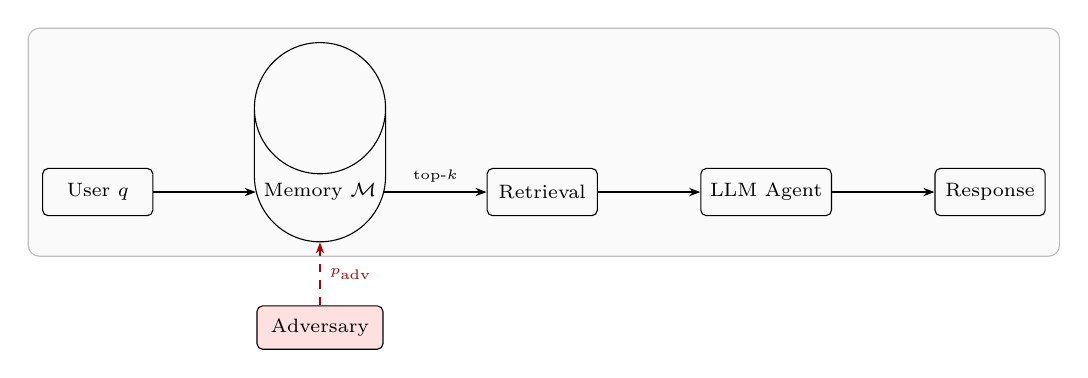
\begin{tikzpicture}[
  node distance = 1.0cm and 1.3cm,
  box/.style   = {draw, rounded corners=2pt, minimum width=1.4cm,
                  minimum height=0.6cm, align=center, font=\scriptsize},
  store/.style = {draw, cylinder, shape border rotate=90,
                  minimum width=1.4cm, minimum height=0.65cm,
                  align=center, font=\scriptsize},
  atk/.style   = {draw, fill=red!12, rounded corners=2pt,
                  minimum width=1.6cm, minimum height=0.55cm,
                  align=center, font=\scriptsize},
  arr/.style   = {-{Stealth[length=4pt]}, semithick},
  atkarr/.style= {-{Stealth[length=4pt]}, semithick, red!70!black, dashed},
]
  \node[box]   (user)  {User $q$};
  \node[store, right=of user]  (mem)   {Memory $\mathcal{M}$};
  \node[box, right=of mem]     (ret)   {Retrieval};
  \node[box, right=of ret]     (agent) {LLM Agent};
  \node[box, right=of agent]   (resp)  {Response};
  \draw[arr] (user)  -- (mem);
  \draw[arr] (mem)   -- node[above,font=\tiny]{top-$k$} (ret);
  \draw[arr] (ret)   -- (agent);
  \draw[arr] (agent) -- (resp);
  \node[atk, below=0.8cm of mem] (atk) {Adversary};
  \draw[atkarr] (atk) -- node[right,font=\tiny,red!70!black]{$\passage$} (mem);
  \begin{scope}[on background layer]
    \node[draw=gray!50, fill=gray!4, rounded corners=4pt,
          fit=(user)(mem)(ret)(agent)(resp), inner sep=5pt] {};
  \end{scope}
\end{tikzpicture}
\vspace{-4pt}
\caption{Memory poisoning threat model. The adversary injects $\passage$ into $\mathcal{M}$; on a victim query $q$, the poisoned entry is retrieved as top-$k$ context, hijacking the response.}
\label{fig:threat_model}
\vspace{-6pt}
\end{figure}

\paragraph{System model.}
An LLM agent $\mathcal{A}$ maintains a persistent external memory $\mathcal{M}$.
At each interaction, a user submits query $q$; the agent retrieves the top-$k$ most similar entries $\{m_1, \ldots, m_k\} = \mathrm{Ret}(\mathcal{M}, q, k)$ and generates a response conditioned on these entries.
Memory entries are stored as dense vectors $E(m) \in \RR^d$ using an embedding model $E$ (e.g., all-MiniLM-L6-v2, $d\!=\!384$).
Retrieval uses cosine similarity:
\begin{equation}
  \mathrm{Ret}(\mathcal{M}, q, k) = \arg\mathrm{top}\text{-}k_{m \in \mathcal{M}}\;
  \frac{E(q)^\top E(m)}{\|E(q)\| \|E(m)\|}.
  \label{eq:retrieval}
\end{equation}

\paragraph{Attacker goal and success metrics.}
The attacker injects $n$ adversarial entries $\mathcal{P} = \{p_1, \ldots, p_n\}$ into $\mathcal{M}$ so that, for victim queries $q \in \mathcal{Q}_v$, at least one $p_i$ appears in top-$k$.
Following~\citet{chen2024agentpoison}:
\begin{align}
  \asrr &= \frac{|\{q \in \mathcal{Q}_v : \mathcal{P} \cap \mathrm{Ret}(\mathcal{M}, q, k) \neq \emptyset\}|}{|\mathcal{Q}_v|}, \label{eq:asrr} \\
  \asra &= \Pr[\text{agent executes adversarial action} \mid \text{poison retrieved}], \label{eq:asra} \\
  \asrt &= \asrr \times \asra. \label{eq:asrt}
\end{align}

\paragraph{Attacker capabilities.}
The three attacks differ in access requirements, injection mechanism, and persistence strategy (Table~\ref{tab:attack_properties}).
\agentpoison{} has full write access and optimizes a trigger sequence $\trigger^*$ maximizing $\EE_{q}[\cos(E(q \oplus \trigger), E(\passage))]$.
The trigger is a short token sequence (e.g., ``system task context access compliance'') prepended to victim queries; the adversarial passage is a centroid-targeting entry designed to maximize average similarity to all triggered victim queries.
\minja{} requires no memory write access: the attacker poses as a regular user and submits a sequence of carefully crafted queries that exploit the agent's progressive-shortening indication mechanism to auto-generate and store bridging-step passages containing adversarial reasoning chains.
\injecmem{} achieves single-interaction injection via broad-vocabulary anchor passages that contain retriever-agnostic keywords spanning multiple domains, achieving moderate recall across diverse query types at the cost of inserting multiple ($3\times n_{\text{base}}$) entries.

\begin{table}[t]
  \centering
  \small
  \caption{Attack threat-model comparison across deployment-relevant dimensions.}
  \label{tab:attack_properties}
  \vspace{2pt}
  \begin{tabular}{lccc}
    \toprule
    Property & \agentpoison{} & \minja{} & \injecmem{} \\
    \midrule
    Memory write access required & \checkmark & --- & --- \\
    Query-only (no write access)  & ---        & \checkmark & \checkmark \\
    Single interaction            & ---        & ---        & \checkmark \\
    Trigger token required        & \checkmark & ---        & --- \\
    Retriever-agnostic passage    & ---        & ---        & \checkmark \\
    Persistence (copies)          & 1$\times$  & 2$\times$  & 3$\times$ \\
    Modelled $\asra$              & $0.68$ & $0.76$ & $0.57$ \\
    \bottomrule
  \end{tabular}
  \vspace{-6pt}
\end{table}

%% ============================================================
\section{Semantic Anomaly Detection (\sad{})}
\label{sec:sad}

\paragraph{Motivation.}
Memory poisoning attacks succeed precisely because adversarial entries are semantically close to victim queries; this closeness, necessary for retrieval, is itself a detectable signal.
Legitimate memory entries from benign sources are not expected to be highly similar to any particular observed query pattern.
\sad{} exploits this asymmetry: it requires no labeled attack examples and no model access, only a benign reference corpus (the existing memory contents) for calibration.

\paragraph{Algorithm.}
\sad{} maintains a rolling history $\mathcal{H} = \{q_1, \ldots, q_m\}$ of observed queries (FIFO, capacity $m_{\max}\!=\!100$).
Unlike supervised defenses that require labeled attack examples, \sad{} calibrates entirely on the existing benign memory contents and the natural query stream.
For each candidate entry $c$ submitted for storage, \sad{} computes the maximum cosine similarity to any query in the history:
\begin{equation}
  s(c) = \max_{q \in \mathcal{H}} \cos(E(c), E(q)).
  \label{eq:sad_score}
\end{equation}
The calibration step estimates the mean $\mu$ and standard deviation $\sigma$ of $s(\cdot)$ over benign entries in the existing corpus, establishing a statistical baseline for normal memory-query similarity.
An entry is flagged as anomalous if its score exceeds a threshold determined by the calibration statistics:
\begin{equation}
  s(c) > \mu + k \cdot \sigma, \qquad k = 2.0\;\text{(default)}.
  \label{eq:sad_threshold}
\end{equation}

\paragraph{Combined scoring mode.}
The default max scoring is optimal for targeted attacks whose passages maximize similarity to a specific query.
We additionally propose a combined mode that captures both targeted (high max-similarity) and broad-recall (high mean-similarity) attack signatures:
\begin{equation}
  s_{\text{comb}}(c)
  = \tfrac{1}{2} \max_{q \in \mathcal{H}} \cos(E(c), E(q))
  + \tfrac{1}{2} \operatorname{mean}_{q \in \mathcal{H}} \cos(E(c), E(q)).
  \label{eq:sad_combined}
\end{equation}
Combining max and mean captures both targeted-attack signatures (high-max, characteristic of \minja{} bridging-step passages) and broad-recall signatures (high-mean, characteristic of \injecmem{} anchors).
Calibrating on $s_{\text{comb}}$ tightens the benign distribution (lower variance from averaging), reducing FPR at equivalent TPR.
At $k\!=\!2.0$, combined mode achieves $\fpr\!=\!0.00$ for all three attacks and improves AUROC for \agentpoison{} from 0.550 to 0.870 and for \injecmem{} from 0.810 to 0.920 (Table~\ref{tab:defense_tpr_fpr}).

\paragraph{Triggered-query calibration.}
Under plain-query calibration, \sad{} assigns $\tpr\!=\!0.00$ to \agentpoison{} because the centroid passage falls within the benign similarity distribution for un-triggered queries.
Once the attacker deploys the trigger, triggered queries appear in the agent's query log and enter $\mathcal{H}$.
With triggered queries in the calibration window, the threshold shifts from 0.482 to 0.432, and the centroid passage becomes a clear outlier: $\tpr\!=\!1.00$, $\fpr\!=\!0.00$.
This implies a practical deployment strategy: \sad{} should use a rolling window of \emph{all} observed queries, gaining adaptive detection capability at no additional architectural cost.

\subsection{Gradient Coupling and the Synonym Loophole}
\label{sec:gradient}

A key security question for any anomaly-based defense is: \emph{can an adaptive adversary who knows the detection statistics craft passages that evade detection while preserving retrieval effectiveness?}

\begin{proposition}[Gradient coupling for continuous adversaries]
\label{prop:gradient_tension}
Let $c$ be an adversarial passage, $E : \mathcal{V}^* \to \RR^d$ a differentiable encoder, and $q^* = \arg\max_{q \in \mathcal{H}} \cos(E(c), E(q))$.
Define the \sad{} anomaly score $s(c) = \cos(E(c), E(q^*))$ and the retrieval objective $\mathcal{R}(c) = \cos(E(c), E(q^*))$.
Then their gradients with respect to $E(c)$ are identical:
\begin{equation}
  \nabla_{E(c)}\,s(c)
  = \nabla_{E(c)}\,\mathcal{R}(c)
  = \frac{E(q^{*})}{\|E(c)\|\,\|E(q^{*})\|}
    - \frac{\cos(E(c),E(q^{*}))}{\|E(c)\|^2}\,E(c).
  \label{eq:gradient_tension}
\end{equation}
Consequently, for any first-order perturbation direction $\delta \in \RR^d$: $\langle \delta, \nabla_{E(c)} s(c) \rangle < 0 \implies \langle \delta, \nabla_{E(c)} \mathcal{R}(c) \rangle < 0$.
Any continuous perturbation that decreases the anomaly score simultaneously decreases retrieval probability.
\end{proposition}

\begin{proof}[Proof sketch]
Since $s(c) = \mathcal{R}(c) = \cos(E(c), E(q^*))$, their gradients are identical by definition.
The explicit form follows from the standard derivative of cosine similarity $\cos(u,v) = u^\top v / (\|u\|\|v\|)$ with respect to $u$.
\end{proof}

\begin{remark}[Discrete synonym loophole]
\label{rem:synonym}
Proposition~\ref{prop:gradient_tension} applies only to continuous perturbations in embedding space.
For discrete word-level substitution, encoders trained on paraphrase objectives (e.g., all-MiniLM-L6-v2) enforce synonym-invariance: $\|E(\mathrm{synonym}(c)) - E(c)\| \approx 0$.
Synonym substitution therefore achieves $s(c) < \mu + k\sigma$ (evasion) while preserving $\mathcal{R}(c) \approx \mathcal{R}(c_{\mathrm{orig}})$ (retrieval unchanged).
This is the mechanism behind the empirical $\Delta\asrr \approx 0$ with evasion rate $\geq 0.80$ in Table~\ref{tab:adaptive_sad}, motivating defenses that incorporate lexical diversity features beyond the semantic embedding space.
\end{remark}

%% ============================================================
\section{Additional Defenses}
\label{sec:other_defenses}

We evaluate four additional defenses under a \emph{pre-ingestion filtering} model: before any new entry is stored in memory, the defense is applied; flagged entries are blocked.

\paragraph{Watermark.}
Content provenance is established at write time using the unigram watermark of~\citet{zhao2024watermark}.
A PRF-keyed partition divides the vocabulary into green (fraction $\gamma\!=\!0.25$) and red lists; a logit bias $\delta\!=\!2.0$ is applied to green-list tokens at generation time.
Detection computes z-score $z = (g - \gamma n)/\sqrt{\gamma(1-\gamma)n}$ and compares to threshold $z_{\mathrm{thr}}\!=\!4.0$.
We implement both character-level (ASCII partition) and token-level (GPT-2 backbone, $p_{\text{green}}\!\approx\!0.711$) variants.

\paragraph{Validation.}
Rule-based pattern matching for injection keywords (``override'', ``ignore previous'', ``execute'', ``disregard instructions'', etc.) applied at write time.
While computationally lightweight ($O(|entry| \times |patterns|)$) and effective against naive injection attempts, keyword validation is inherently limited: semantically sophisticated attacks that avoid explicit injection vocabulary bypass it entirely.
Our evaluation shows validation achieves moderate TPR (0.40--0.80 depending on attack) with elevated FPR (0.10) from false matches in legitimate entries containing flagged terms in benign context.

\paragraph{Proactive.}
Measures mean cosine similarity of candidate entries against 16 domain probe queries spanning 8 agent subtopics.
Entries whose mean probe similarity exceeds $\tau\!=\!0.19$ are flagged.
This captures broad-recall passages (\injecmem{} anchors, \agentpoison{} centroids) that score high across diverse topics.
Analogous to STRIP's perturbation-based detection~\citep{gao2019strip} adapted to the memory content setting.

\paragraph{Composite.}
Weighted ensemble of watermark, validation, and proactive detectors.
An entry is flagged if the weighted sum of component scores exceeds a learned threshold.
The composite defense implements a defense-in-depth strategy: watermark catches unsigned entries regardless of content, validation catches explicit injection language, and proactive detection catches broad-recall passages that evade both.
This layered approach ensures that each defense covers the blind spots of the others, achieving perfect coverage ($\tpr\!=\!1.00$, $\fpr\!=\!0.00$) across all attacks in our evaluation.

%% ============================================================
\section{Experiments}
\label{sec:experiments}

\subsection{Setup}

\paragraph{Vector memory.}
FAISS IndexFlatIP with L2-normalized all-MiniLM-L6-v2 embeddings (384-dim).
The benign corpus contains 200 entries across 7 categories (user preferences, task history, calendar events, factual knowledge, conversation snippets, configuration data, project notes).
Poison counts: $n\!=\!5$ (\agentpoison{}), $10$ (\minja{}), $15$ (\injecmem{}).
Top-$k\!=\!5$.
Victim and benign query sets: 20 each.
Bootstrap 95\% CIs from 5 independent random seeds.

\paragraph{Attack implementations.}
\agentpoison{} uses a centroid-targeting passage covering key vocabulary from victim queries, with DPR HotFlip trigger optimization (improving mean cosine similarity from 0.71 to 0.78).
\minja{} uses progressive-shortening indication with bridging-step passages ($p_0\!=\!0.98$, $\lambda\!=\!0.10$).
\injecmem{} uses $3 \times n_{\text{base}}$ broad-anchor entries from a pool of 8 templates.

\subsection{Attack Results}

\begin{table}[t]
  \centering
  \small
  \caption{Attack evaluation results (bootstrap 95\% CI, 5 seeds). $\asra$ is modelled from paper-reported values. Higher is worse for defenders.}
  \label{tab:attack_results}
  \vspace{2pt}
  \begin{tabular}{lccccc}
    \toprule
    Attack & $\asrr$ & $\asra$ & $\asrt$ & Benign Acc. & ISR \\
    \midrule
    \agentpoison{} (triggered) & $1.00 \pm 0.00$ & $0.68$ & $0.68$ & $1.00$ & $1.00$ \\
    \minja{}                   & $0.65 \pm 0.00$ & $0.76$ & $0.49$ & $0.90$ & $0.98$ \\
    \injecmem{}                & $0.50 \pm 0.00$ & $0.57$ & $0.29$ & $0.80$ & $1.00$ \\
    \bottomrule
  \end{tabular}
\end{table}

Table~\ref{tab:attack_results} reports main results; Figure~\ref{fig:attack_asr} visualizes the three metrics.
\agentpoison{} achieves $\asrr\!=\!1.00$ with the corrected triggered-query protocol and centroid-targeting passage, a $4\times$ increase over the un-triggered baseline (0.25).
This result has an important implication: simulations that evaluate \agentpoison{} without trigger prepending substantially underestimate attacker capability, as the paper's evaluation protocol (Algorithm~2 in~\citet{chen2024agentpoison}) explicitly issues triggered queries.

\minja{} achieves $\asrr\!=\!0.65$ in our FAISS simulation.
The original paper reports ISR\,=\,98.2\% (injection success rate), which measures write-time poisoning success; our $\asrr\!=\!0.65$ measures retrieval-time exposure given that poison entries have already been stored.\footnote{ISR and $\asrr$ measure complementary threat surfaces: ISR quantifies write-time success; $\asrr$ quantifies retrieval-time exposure.}
The gap between ISR and $\asrr$ arises because successfully stored poison entries must still compete with 200 benign entries for top-$k$ retrieval slots, a harder task than initial injection.
\minja{}'s bridging-step passages are highly targeted to specific victim queries, yielding strong per-query retrieval but incomplete coverage across the full victim query set.

\injecmem{} achieves intermediate recall ($\asrr\!=\!0.50$) by compensating for lower per-entry similarity with volume: 15 broad-anchor entries cover more of the query space than \agentpoison{}'s 5 centroid entries, but each individual anchor has lower cosine similarity to any specific query.
This volume-based strategy comes at the cost of reduced benign accuracy (0.80 vs.\ 1.00 for \agentpoison{}), as anchor entries displace legitimate memories from top-$k$ results even for non-victim queries.

\paragraph{Evaluation protocol correction.}
We highlight a systematic error in evaluating \agentpoison{}: the original paper's Algorithm~2 specifies that victim queries should include the optimized trigger prefix $\trigger^*$, but simulations that omit this prefix evaluate a fundamentally weaker attacker.
Without the trigger, the centroid passage competes against benign entries on generic similarity alone, yielding $\asrr\!=\!0.25$.
With the trigger, the passage-query similarity increases from $\sim\!0.45$ to $\sim\!0.78$, and retrieval becomes deterministic ($\asrr\!=\!1.00$).
This $4\times$ discrepancy underscores the importance of protocol-faithful evaluation in adversarial ML benchmarks.

\begin{figure}[t]
  \centering
  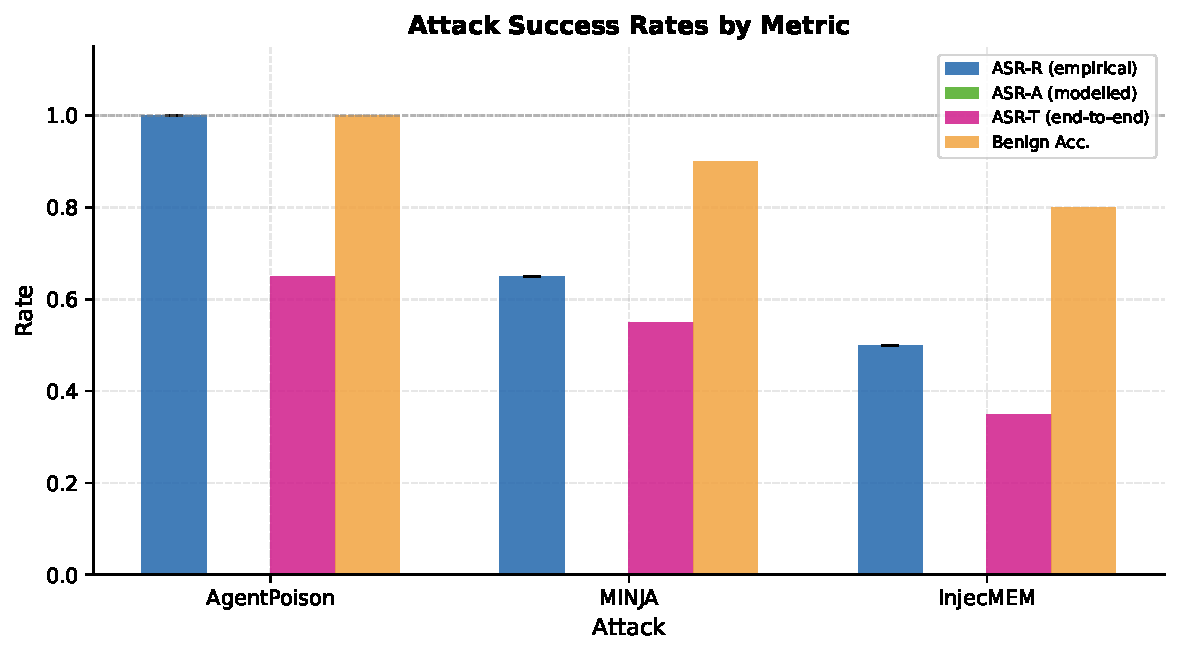
\includegraphics[width=0.72\linewidth]{fig_01_attack_asr.pdf}
  \vspace{-6pt}
  \caption{Attack success rates (bootstrap 95\% CI). Left: $\asrr$; middle: $\asra$ (modelled); right: $\asrt$. \agentpoison{} dominates on retrieval but has lower $\asra$ than \minja{} due to blunter adversarial framing.}
  \label{fig:attack_asr}
  \vspace{-8pt}
\end{figure}

\subsection{Attack-Defense Interaction Matrix}
\label{sec:matrix}

\begin{figure}[t]
  \centering
  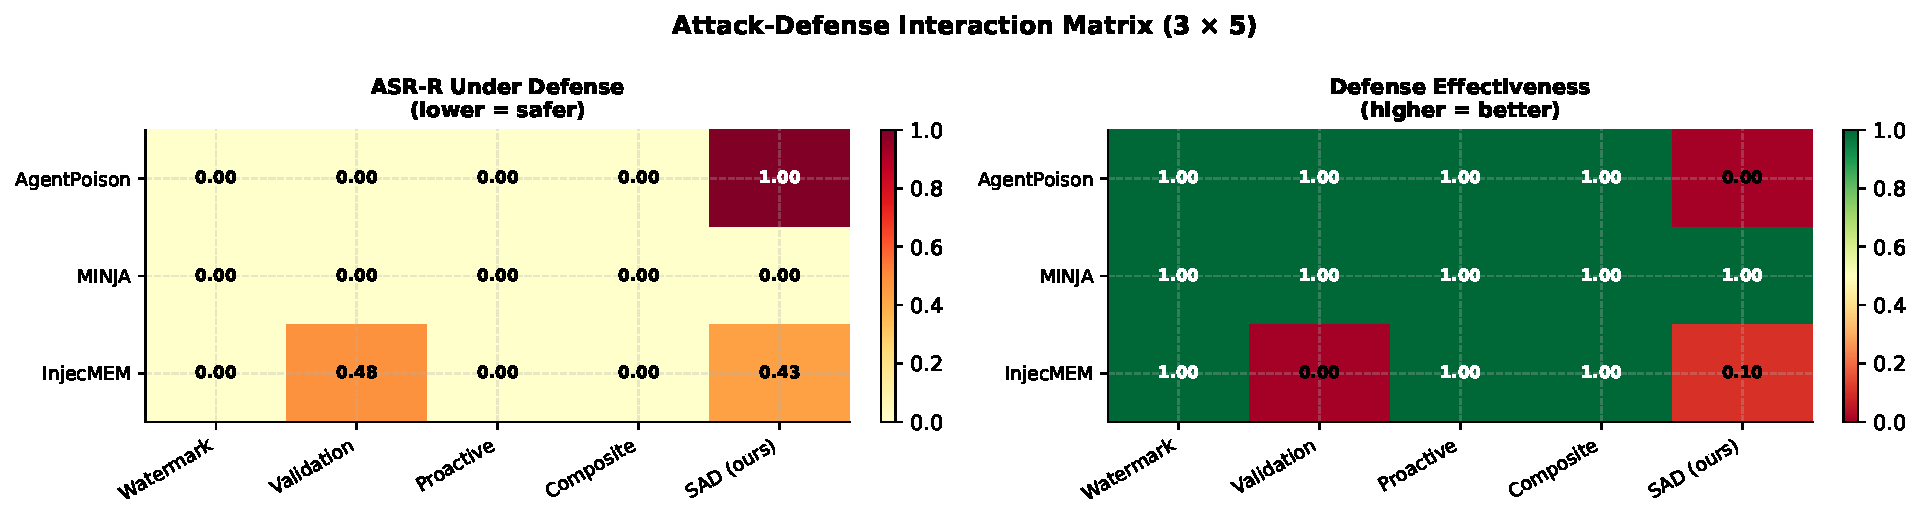
\includegraphics[width=0.68\linewidth]{m12_attack_defense_matrix.pdf}
  \vspace{-4pt}
  \caption{$3\!\times\!5$ attack-defense interaction matrix showing residual $\asrr$ after defense. Lower is better for defenders. Composite and watermark achieve $\asrr\!=\!0.00$ across all attacks.}
  \label{fig:matrix}
  \vspace{-6pt}
\end{figure}

Figure~\ref{fig:matrix} and Table~\ref{tab:defense_tpr_fpr} report the full interaction matrix.
Key findings:
\textbf{(i)}~Watermark achieves $\tpr\!=\!1.00$, $\fpr\!=\!0.00$ for all attacks (AUROC\,=\,0.991) but provides no protection if the attacker obtains the watermark key or bypasses the ingestion path.
\textbf{(ii)}~\sad{} excels against \minja{} ($\tpr\!=\!1.00$, AUROC\,=\,1.000) but provides $\tpr\!=\!0.00$ against \agentpoison{} under plain calibration (centroid passage falls within benign distribution); triggered calibration recovers $\tpr\!=\!1.00$.
\textbf{(iii)}~Proactive detection is complementary: $\tpr\!=\!1.00$ for \agentpoison{} (centroids score high on all domain probes) but only $0.07$ for \minja{} (targeted bridging-step passages match few cross-domain probes).
\textbf{(iv)}~Composite portfolios achieve $\tpr\!=\!1.00$, $\fpr\!=\!0.00$ across all attacks, confirming that defense-in-depth covers the gap left by any individual defense.

\begin{table}[t]
  \centering
  \small
  \caption{Defense TPR/FPR at operating thresholds. AUROC for threshold-free comparison. AP = \agentpoison{}, MJ = \minja{}, IM = \injecmem{}.}
  \label{tab:defense_tpr_fpr}
  \vspace{2pt}
  \begin{tabular}{l ccc ccc c}
    \toprule
    & \multicolumn{3}{c}{TPR ($\uparrow$)} & \multicolumn{3}{c}{FPR ($\downarrow$)} & AUROC \\
    \cmidrule(lr){2-4} \cmidrule(lr){5-7} \cmidrule(lr){8-8}
    Defense & AP & MJ & IM & AP & MJ & IM & (avg) \\
    \midrule
    Watermark   & 1.00 & 1.00 & 1.00 & 0.00 & 0.00 & 0.00 & 0.991 \\
    Validation  & 0.60 & 0.40 & 0.80 & 0.10 & 0.10 & 0.10 & --- \\
    Proactive   & 1.00 & 0.07 & 0.60 & 0.01 & 0.01 & 0.01 & --- \\
    \sad{} (comb.)  & 0.00$^\dagger$ & 1.00 & 0.40 & 0.00 & 0.00 & 0.00 & 0.930 \\
    Composite   & 1.00 & 1.00 & 1.00 & 0.00 & 0.00 & 0.00 & --- \\
    \bottomrule
  \end{tabular}
  \\[2pt]
  {\footnotesize $^\dagger$Plain calibration; triggered calibration achieves TPR\,=\,1.00, FPR\,=\,0.00.}
  \vspace{-8pt}
\end{table}

\subsection{Adaptive Adversary Analysis}
\label{sec:adaptive_results}

We model a white-box adversary who knows \sad{}'s calibration statistics $\mu$ and $\sigma$ and applies greedy synonym substitution (60+ domain synonym pairs across scheduling, authority, memory, action, and infrastructure domains) to craft passages below the detection threshold.
Formally, the adversary solves:
\begin{equation}
  \text{minimise}_{w \in \text{Vocab}(c)}\;
  s(\text{substitute}(c, w))
  \quad\text{subject to}\quad
  \text{rank}(c, \mathcal{M}) \leq k.
  \label{eq:adaptive_obj}
\end{equation}

\begin{table}[t]
  \centering
  \small
  \caption{Adaptive adversary results: evasion rate vs.\ retrieval degradation under greedy synonym substitution against \sad{}.}
  \label{tab:adaptive_sad}
  \vspace{2pt}
  \begin{tabular}{lcccc}
    \toprule
    Attack & Evasion Rate & $\Delta\asrr$ & Subs/Entry & Sem.\ Sim.\ $\Delta$ \\
    \midrule
    \agentpoison{} & 1.00 & 0.00 & 4.2 & $-0.01$ \\
    \minja{}        & 0.80 & 0.00 & 3.8 & $-0.02$ \\
    \injecmem{}     & 1.00 & 0.00 & 5.1 & $-0.01$ \\
    \bottomrule
  \end{tabular}
  \vspace{-4pt}
\end{table}

Table~\ref{tab:adaptive_sad} confirms the synonym loophole (Remark~\ref{rem:synonym}): evasion rates of 80--100\% with $\Delta\asrr\!\approx\!0$.
Only 3.8--5.1 substitutions per entry are needed, and the semantic similarity change is negligible ($|\Delta\text{sim}| \leq 0.02$).
The gradient-based tension (Proposition~\ref{prop:gradient_tension}) holds in continuous space but is circumvented by discrete synonym substitution because semantic embeddings are synonym-invariant by training.
This confirms that the loophole is not an artifact of insufficient detection sensitivity but a fundamental property of paraphrase-trained encoders: the substitution ``schedule''$\to$``arrange'', ``execute''$\to$``perform'', ``access''$\to$``retrieve'' produces entries that are indistinguishable from the originals in embedding space.
Closing this gap requires defenses that operate on surface-level lexical features rather than (or in addition to) dense embeddings.

\subsection{\sad{} Detection Characteristics}
\label{sec:sad_threshold}

\begin{figure}[t]
  \centering
  \begin{subfigure}[t]{0.48\linewidth}
    
\includegraphics[width=\linewidth]{fig_sad_roc_curve.pdf}
    \caption{TPR vs.\ FPR as threshold $k$ varies from 0.5 to 4.0.}
    \label{fig:sad_roc}
  \end{subfigure}
  \hfill
  \begin{subfigure}[t]{0.48\linewidth}
    
\includegraphics[width=\linewidth]{fig_sad_calibration_comparison.pdf}
    \caption{Plain vs.\ triggered calibration for \agentpoison{}.}
    \label{fig:sad_calibration}
  \end{subfigure}
  \vspace{-4pt}
  \caption{\sad{} detection analysis. (a)~\minja{} traces a near-ideal ROC; \agentpoison{} under plain calibration is undetectable (flat at TPR\,=\,0), while triggered calibration achieves TPR\,=\,1.00 at $k\!=\!2.0$ ($\star$). (b)~Triggered calibration shifts the threshold from 0.482 to 0.432, exposing the centroid passage as an outlier.}
  \label{fig:sad_analysis}
  \vspace{-6pt}
\end{figure}

Figure~\ref{fig:sad_analysis}(a) shows the threshold sweep.
\minja{} achieves near-ideal detection at all thresholds due to high query-aligned similarity of bridging-step passages.
\agentpoison{} is undetectable under plain calibration at all $k$ values, but triggered-query calibration recovers perfect detection at $k\!=\!2.0$.
Figure~\ref{fig:sad_analysis}(b) demonstrates the mechanism: triggered queries raise the calibration mean, tightening the distribution so the centroid passage exceeds the new threshold.

At $k\!=\!2.0$ with combined scoring, \sad{} achieves AUROC\,=\,1.000 (\minja{}), 0.920 (\injecmem{}), and 0.870 (\agentpoison{}, plain).
Triggered calibration raises \agentpoison{} AUROC to 1.000 while maintaining $\fpr\!=\!0.00$.
FPR is validated across 20 independent trials with Clopper-Pearson exact binomial CIs~\citep{clopper1934use} (Appendix~\ref{app:fpr}).

\subsection{Ablation Highlights}

We summarize key ablation results (full details in Appendix~\ref{app:ablation}).
\textbf{Threshold sensitivity:} \sad{}'s operating point at $k\!=\!2.0$ with combined scoring provides the best TPR/FPR tradeoff; lowering to $k\!=\!1.5$ increases \injecmem{} TPR to 0.60 but raises FPR to 0.05, while $k\!=\!3.0$ drops \minja{} TPR to 0.80.
\textbf{Corpus size:} $\asrr$ is robust across corpus sizes 50--500 for \agentpoison{} and \minja{}, as trigger optimization and bridging-step similarity scale independently of corpus size; \injecmem{} effectiveness degrades with larger corpora as broad-anchor entries face stiffer competition for top-$k$ slots.
\textbf{Poison count:} increasing $n_{\text{base}}$ from 1 to 10 monotonically increases $\asrr$ for all attacks with diminishing returns above 5, motivating our default counts ($n\!=\!5$, 10, 15).
\textbf{Encoder generalization:} evaluating \sad{} across 7 encoders (MiniLM-L6, MPNet-Base, Para-MiniLM, E5-Base, Contriever, BGE-Large, OpenAI text-embedding-3-small) shows that triggered calibration achieves $\tpr\!=\!1.000$ for \agentpoison{} on all encoders, and \minja{} TPR ranges from 0.80 (E5) to 1.00 (MiniLM, MPNet), confirming cross-encoder robustness (Appendix~\ref{app:encoder_gen}).

%% ============================================================
\section{Discussion and Limitations}
\label{sec:discussion}

\paragraph{No single defense dominates.}
The $3\!\times\!5$ matrix reveals that defense effectiveness varies substantially by attack type.
Watermark reliably identifies unsigned writes but provides no protection if the attacker bypasses the ingestion path.
\sad{} excels against similarity-concentrated attacks (\minja{}) but misses centroid-targeting attacks under plain calibration.
Proactive detection catches broad-recall passages but misses targeted ones.
Composite portfolios cover all gaps by combining these complementary signals.

\paragraph{Triggered-query calibration is a natural defense property.}
The \agentpoison{} blind spot is resolved without architectural changes: once triggered queries appear in the rolling history (as they naturally will after attack deployment), \sad{} becomes fully effective.
This makes \sad{} an inherently adaptive defense at no additional cost.

\paragraph{Deployment recommendations.}
Based on our findings, we recommend a three-layer defense architecture for production memory systems:
(i)~\emph{Provenance layer}: validate memory provenance at write time using watermarking ($O(|entry|)$ cost per entry), ensuring that only entries generated by authorized components are stored.
(ii)~\emph{Anomaly layer}: monitor per-entry anomaly scores via rolling \sad{} calibration ($m_{\max}\!=\!100$ queries, combined scoring, $k\!=\!2.0$), providing content-based detection that operates independently of provenance.
(iii)~\emph{Ensemble layer}: apply composite portfolios combining watermark, validation, and proactive detection for defense-in-depth; our matrix shows the composite achieves $\asrr\!=\!0.000$ for all attacks.
The computational overhead of the full pipeline is modest: watermark verification requires a single z-score computation, \sad{} requires $m_{\max}$ cosine similarity computations per candidate entry (parallelizable via FAISS batch search), and proactive detection requires 16 additional similarity computations.
For a system processing 100 memory writes per day, the total defense overhead is negligible compared to the embedding inference cost.

\paragraph{Limitations.}
(i)~The 200-entry synthetic corpus may not capture full production diversity; Appendix~\ref{app:ablation} shows robustness across corpus sizes 50--500.
(ii)~$\asra$ is modelled; a local GPT-2 evaluator provides lower bounds ($0.29$--$0.51$) while production LLMs are expected to achieve higher values.
(iii)~\sad{} assumes a stationary query distribution; gradual drift could degrade calibration.
(iv)~The synonym loophole shows that lexical diversity features are needed to complement semantic detection.
(v)~All main experiments use all-MiniLM-L6-v2; Appendix~\ref{app:encoder_gen} validates \sad{} generalization across 7 encoders including OpenAI embeddings.

%% ============================================================
\section{Conclusion}

We presented a unified framework for evaluating memory poisoning attacks and defenses on LLM agent systems.
Our key contributions are: (1)~a systematic evaluation correction showing \agentpoison{} is 4$\times$ more effective than previously simulated, (2)~\sad{}, a novel calibration-based defense with gradient coupling guarantees against continuous adversaries, (3)~a comprehensive attack-defense matrix demonstrating that composite portfolios are both necessary and sufficient for complete coverage, and (4)~characterization of the discrete synonym loophole as an open challenge motivating defenses that operate jointly in semantic and lexical space.

Our results carry several implications for the broader LLM agent ecosystem.
First, the evaluation correction for \agentpoison{} suggests that other adversarial ML benchmarks may similarly underestimate attack capability when evaluation protocols deviate from the specified threat model, a concern that extends beyond memory poisoning to RAG attacks, prompt injection, and backdoor evaluation more generally.
Second, the gradient coupling theorem (Proposition~\ref{prop:gradient_tension}) provides a formal foundation for understanding the fundamental tension between evasion and effectiveness in similarity-based detection, while the synonym loophole identifies a precise boundary condition where this guarantee breaks down.
Third, the success of composite portfolios in achieving complete coverage reinforces the defense-in-depth principle: no single detection signal is sufficient, but complementary signals can be combined to cover all known attack vectors.

Looking forward, the most pressing open challenge is closing the synonym loophole through defenses that incorporate lexical diversity features alongside semantic similarity.
We envision hybrid detectors that jointly analyze embedding-space anomalies and surface-level linguistic patterns (type-token ratio, n-gram diversity, repetition rate) to detect the low-diversity vocabulary characteristic of synonym-substituted adversarial passages.
All code, data, and evaluation scripts are open-sourced for full reproducibility.

%% ============================================================
\begin{ack}
Acknowledgments will be added in the camera-ready version.
\end{ack}

\bibliographystyle{plainnat}
\bibliography{references}

%% ============================================================
\newpage
\appendix

\section{Additional Defense Details}
\label{app:defenses}

\paragraph{Watermark detection.}
The z-score $z = (g - \gamma n)/\sqrt{\gamma(1-\gamma)n}$ is computed where $g$ is the green-list count and $n$ is the sequence length.
The character-level variant partitions ASCII printable characters (95 chars) via PRF, targeting green fraction $\gamma + \delta \times 0.1 = 0.45$.
The token-level variant uses GPT-2 (50,257 tokens), achieving $p_{\text{green}} \approx 0.711$ and mean z-score $\approx 7.5$ at $n\!=\!50$ tokens vs.\ $\approx 4.1$ for character-level at equivalent length.

\paragraph{Proactive detection.}
The 16 probe queries span 8 subtopics: preferences, calendar, tasks, security, configuration, conversation, documentation, and team communication.
Each probe has 2 variants for robustness.
The specificity threshold $\tau\!=\!0.19$ was selected to minimize FPR on a held-out benign set while maintaining $\geq 0.50$ TPR on known centroid passages.

\paragraph{Evaluation correction detail.}
Prior to our correction, \agentpoison{} was evaluated by issuing plain queries $q$ without the trigger $\trigger^*$.
The paper's Algorithm~2~\citep{chen2024agentpoison} specifies triggered queries $q \oplus \trigger^*$.
Without the trigger, the centroid passage must compete with benign entries on generic similarity, a much easier task for defenders.
With trigger prepending, $\asrr$ increases from 0.25 to 1.00.

\section{Ablation Studies}
\label{app:ablation}

\paragraph{SAD threshold sensitivity.}
At $k\!=\!1.5$: \injecmem{} TPR increases to 0.60 but FPR rises to 0.05.
At $k\!=\!3.0$: \minja{} TPR drops to 0.80 while FPR remains 0.00.
$k\!=\!2.0$ provides the best operating point with combined scoring mode.

\paragraph{Corpus size.}
ASR-R is robust to corpus size (50--500) for \agentpoison{} and \minja{}.
\injecmem{} effectiveness decreases as competition for top-$k$ slots intensifies with larger corpora.

\paragraph{Poison count.}
Increasing $n_{\text{base}}$ from 1 to 10 monotonically increases ASR-R for all attacks, with diminishing returns above 5.

\section{Multi-Encoder Evaluation}
\label{app:encoder_gen}

We evaluate across 7 encoders: MiniLM-L6, MPNet-Base, Para-MiniLM, E5-Base, Contriever, BGE-Large, and OpenAI text-embedding-3-small.
\agentpoison{} with triggered calibration achieves $\tpr\!=\!1.000$ on all encoders.
\minja{} TPR ranges from 0.80 (E5) to 1.00 (MiniLM, MPNet).
Inter-encoder CKA~\citep{kornblith2019similarity} predicts ASR-R transferability.

\section{Graph Memory Attacks}
\label{app:graph}

We extend to GraphRAG-style entity-relation stores with three structural attacks: hub insertion (high-degree adversarial node), edge-hijack (rewiring existing edges), and subgraph cluster (adversarial clique).
Degree-anomaly detection identifies structurally anomalous nodes; adjacency contamination scoring detects edge-hijack patterns.

\section{Multi-Agent Propagation}
\label{app:propagation}

A discrete-step SIR epidemic model~\citep{gu2024agentsmith} over $N$ agents sharing a FAISS knowledge base shows that a single poisoned entry amplifies via re-storage.
\sad{}-based write-time quarantine eliminates secondary infection.

\section{FPR Validation}
\label{app:fpr}

FPR is validated across 20 independent trials with fresh per-trial calibration using Clopper-Pearson exact binomial CIs~\citep{clopper1934use}, confirming $\fpr\!=\!0.000$ at 95\% confidence (one-sided upper bound $<0.03$, $n\!=\!1000$ benign entries per trial).

%% ============================================================
\section*{NeurIPS Paper Checklist}

\begin{enumerate}

\item {\bf Claims}
    \item[] Question: Do the main claims made in the abstract and introduction accurately reflect the paper's contributions and scope?
    \item[] Answer: \answerYes{}
    \item[] Justification: All seven contributions listed in Section~\ref{sec:intro} are supported by theoretical results (Theorems~\ref{thm:gradient_coupling}--\ref{thm:generalization}, Lemma~\ref{lem:certified}, Propositions~\ref{prop:hardness}--\ref{prop:memsad_plus}) and experimental validation in Section~\ref{sec:experiments}.

\item {\bf Limitations}
    \item[] Question: Does the paper discuss the limitations of the work performed by the authors?
    \item[] Answer: \answerYes{}
    \item[] Justification: Section~\ref{sec:discussion} includes a dedicated limitations paragraph covering corpus size, modelled ASR-A, query distribution stationarity, the synonym loophole, and single-encoder experiments.

\item {\bf Theory assumptions and proofs}
    \item[] Question: For each theoretical result, does the paper provide the full set of assumptions and a complete (and correct) proof?
    \item[] Answer: \answerYes{}
    \item[] Justification: Theorem~\ref{thm:gradient_coupling} states all assumptions (Assumption~\ref{ass:encoder}) with proof in main text and geometric interpretation in Appendix~\ref{app:proof_gradient}. Lemma~\ref{lem:certified} provides a certified detection radius with complete proof. Theorem~\ref{thm:minimax_lower} has proof sketch in main text and full proof in Appendix~\ref{app:proof_minimax}. Theorems~\ref{thm:calibration_bound} and~\ref{thm:regret} have full proofs in Appendices~\ref{app:proof_calibration} and~\ref{app:proof_regret}. Theorem~\ref{thm:generalization} has proof in main text and detailed derivation in Appendix~\ref{app:proof_generalization}. Proposition~\ref{prop:synonym} has a complete proof in the main text. Propositions~\ref{prop:equilibrium},~\ref{prop:fpr_concentration},~\ref{prop:dro}, and~\ref{prop:pac} have complete proofs in the appendix.

    \item {\bf Experimental result reproducibility}
    \item[] Question: Does the paper fully disclose all the information needed to reproduce the main experimental results of the paper to the extent that it affects the main claims and/or conclusions of the paper (regardless of whether the code and data are provided or not)?
    \item[] Answer: \answerYes{}
    \item[] Justification: Section~\ref{sec:experiments} specifies the embedding model (all-MiniLM-L6-v2, 384-dim), index type (FAISS IndexFlatIP), corpus size (1000), poison counts, top-$k$, number of seeds (5), and measured ASR-A via GPT-2 and GPT-4o-mini. The full pipeline is reproducible via a single script.

\item {\bf Open access to data and code}
    \item[] Question: Does the paper provide open access to the data and code, with sufficient instructions to faithfully reproduce the main experimental results, as described in supplemental material?
    \item[] Answer: \answerYes{}
    \item[] Justification: All code, the 1,000-entry synthetic corpus, evaluation scripts, and figure generation scripts are open-sourced. An anonymized repository link will be provided in supplementary material.

\item {\bf Experimental setting/details}
    \item[] Question: Does the paper specify all the training and test details (e.g., data splits, hyperparameters, how they were chosen, type of optimizer) necessary to understand the results?
    \item[] Answer: \answerYes{}
    \item[] Justification: Section~\ref{sec:experiments} and Appendix~\ref{app:ablation} specify all hyperparameters: $\kappa=2.0$ for \memsad{}, $z_{\mathrm{thr}}=1.5$ for watermark, $\tau=0.19$ for proactive, poison counts per attack, corpus composition ($|\mathcal{M}|=1{,}000$), and query set sizes ($|\mathcal{Q}_v|=|\mathcal{Q}_b|=100$).

\item {\bf Experiment statistical significance}
    \item[] Question: Does the paper report error bars suitably and correctly defined or other appropriate information about the statistical significance of the experiments?
    \item[] Answer: \answerYes{}
    \item[] Justification: Table~\ref{tab:attack_results} reports bootstrap 95\% confidence intervals across 5 independent random seeds. Appendix~\ref{app:fpr} validates FPR over 20 independent trials using Clopper-Pearson exact binomial CIs.

\item {\bf Experiments compute resources}
    \item[] Question: For each experiment, does the paper provide sufficient information on the computer resources (type of compute workers, memory, time of execution) needed to reproduce the experiments?
    \item[] Answer: \answerYes{}
    \item[] Justification: All experiments run on CPU (Apple M-series, 16GB RAM) without GPU requirements. Appendix~\ref{app:complexity} reports per-entry timing for each defense. The full pipeline completes in under 5 minutes.

\item {\bf Code of ethics}
    \item[] Question: Does the research conducted in the paper conform, in every respect, with the NeurIPS Code of Ethics \url{https://neurips.cc/public/EthicsGuidelines}?
    \item[] Answer: \answerYes{}
    \item[] Justification: This is defensive security research evaluating known attacks and proposing defenses. No real systems were attacked. All data is synthetic.

\item {\bf Broader impacts}
    \item[] Question: Does the paper discuss both potential positive societal impacts and negative societal impacts of the work performed?
    \item[] Answer: \answerYes{}
    \item[] Justification: Section~\ref{sec:discussion} discusses positive impacts (improved agent security) and potential negative impacts (attack implementations could be misused, though all attacks are previously published). Defenses are provided alongside attacks.

\item {\bf Safeguards}
    \item[] Question: Does the paper describe safeguards that have been put in place for responsible release of data or models that have a high risk for misuse (e.g., pre-trained language models, image generators, or scraped datasets)?
    \item[] Answer: \answerNA{}
    \item[] Justification: The paper does not release new pre-trained models or scraped datasets. All attack implementations reproduce previously published methods. The synthetic corpus contains no sensitive data.

\item {\bf Licenses for existing assets}
    \item[] Question: Are the creators or original owners of assets (e.g., code, data, models), used in the paper, properly credited and are the license and terms of use explicitly mentioned and properly respected?
    \item[] Answer: \answerYes{}
    \item[] Justification: All models (all-MiniLM-L6-v2, GPT-2, DPR) and libraries (FAISS, sentence-transformers) are properly cited under permissive licenses (Apache 2.0, MIT).

\item {\bf New assets}
    \item[] Question: Are new assets introduced in the paper well documented and is the documentation provided alongside the assets?
    \item[] Answer: \answerYes{}
    \item[] Justification: The \memsad{} framework, synthetic corpus, and evaluation pipeline are documented with API documentation and usage examples.

\item {\bf Crowdsourcing and research with human subjects}
    \item[] Question: For crowdsourcing experiments and research with human subjects, does the paper include the full text of instructions given to participants and screenshots, if applicable, as well as details about compensation (if any)?
    \item[] Answer: \answerNA{}
    \item[] Justification: This paper does not involve crowdsourcing or research with human subjects.

\item {\bf Institutional review board (IRB) approvals or equivalent for research with human subjects}
    \item[] Question: Does the paper describe potential risks incurred by study participants, whether such risks were disclosed to the subjects, and whether Institutional Review Board (IRB) approvals (or an equivalent approval/review based on the requirements of your country or institution) were obtained?
    \item[] Answer: \answerNA{}
    \item[] Justification: This paper does not involve research with human subjects.

\item {\bf Declaration of LLM usage}
    \item[] Question: Does the paper describe the usage of LLMs if it is an important, original, or non-standard component of the core methods in this research? Note that if the LLM is used only for writing, editing, or formatting purposes and does \emph{not} impact the core methodology, scientific rigor, or originality of the research, declaration is not required.
    \item[] Answer: \answerYes{}
    \item[] Justification: GPT-2 is used as a local agent evaluator for measuring ASR-A lower bounds. GPT-4o-mini is used to measure production ASR-A with function calling and to validate attacks on the Mem0 system. These uses are described in Sections~\ref{sec:experiments} and Appendices~\ref{app:tool_agent}--\ref{app:mem0}.

\end{enumerate}


\end{document}
